\documentclass{article}
\usepackage{times}
\usepackage[nohead,bottom=3cm,top=2cm,a4paper]{geometry}
\usepackage[table]{xcolor}
%\usepackage{xcolor,colortbl}
\usepackage{graphicx}
\usepackage[nswissgerman]{babel}
\usepackage{listings}
\usepackage{blindtext}
\usepackage{lipsum}
\usepackage{tikz}
\usepackage{float}
\usetikzlibrary{positioning}
\usepackage{amssymb}    % math symbols
\usepackage{amsmath}    % math symbols
\graphicspath{ {./results/} }
\usetikzlibrary{shadows,matrix} % Shadows for nodes
\usetikzlibrary{arrows.meta}
\title{Report aus dem Projekt sensor Cube}
\newlength\mylength
\setlength\mylength{\dimexpr.42\columnwidth-2\tabcolsep-0.42\arrayrulewidth\relax}
	
\definecolor{Gray}{gray}{0.9}

\author{von Ugur Turhal, Berkan Kurt \& Silvan Lenzlinger}
\begin{document}
\maketitle
\abstract{Dieses Report Dokument ist im Rahmen der Vorlesung, Rechenarchitektur \& vertrauenwürdiges Rechnen entstanden. Das Ziel war ein 4 x 4 x 4  Kubus zu löten. Diesen mit einem digitalen Luftfeuchtigskeits-\& Temperatursensor zu verbinden. Dieser soll anhand der idealen Luftfeuchtigkeit und der richtigen Temperatur, für den Schlaf, erreicht ist, spezifische Muster ausgeben.}
%%%%
\section{Einleitung}
Als wir im November uns als Team zusammengesetzt haben war die Mission sofort klar. Wir wollten mit dem Projekt etwas schaffen, welches uns im alltäglichen Leben auch über den Projektzeitraum hinaus, begleiten soll.
Nach reichlicher Überlegung entschieden wir uns für das Oberthema Schlaf. Wir haben den Schlaf gewählt, weil uns aufgefallen ist, dass wir alle drei unseren Schlaf als minderwertig beurteilen. Als wir uns über die Ursachen und Gründe für unseren schlechten Schlaf ausgetauscht haben, kamen wir zum Entschluss, dass wir uns mit der Optimalen Raumtemperatur nie auseinandergesetzt haben. Diese ist vor allem im Winter wichtig, da die Raumtemperatur sich zu dieser Jahreszeit oftmals über der optimalen Raumtemperatur, bedingt durch das Überheizen, befindet.
Im Nachfolgenden Report werden wir darüber reden, wie wir ein Gadget erstellt haben, welches uns hilft, dieses Problem zu lösen.

\section{Aufteilung}

\section{Jigs/Werkzeuge}
Als Jigs werden Hilfsmittel bezeichnet, die beim Prozess des Fertigstellen das Leben vereinfachen. 
\begin{itemize}
\item Ein Raster aus Holz, in welcher die LEDs reingestellt wurden und verlötet wurden.
\item  Ein Holzbrett mit welchem die Anode und Kathode in die nötige formgebracht wurden.
\item Eine Bohrmaschine, welche das Kupferdraht gerade Gewickelt hat.
\item Ein Gerät das den Kupferdraht hielt.   
\end{itemize}
Die folgenden Werkzeuge wurden für die Kommunikation und als Austausch verwendet.
\begin{itemize}
\item GitHub, sorgte für einen Reibungslosen Code und einen Austausch.
\item WhatsApp, auf welchem die Meetings festgelegt wurden.
\item Zoom, bei Meetings, wenn jemand nicht Anwesend war oder für Diskussion.
\item \LaTeX \text{ }dort wurden alle Dokumente erfasst.
\end{itemize} 
\section{Sammeln der Daten}
Bevor das Projekt begann hat Ugur, für die Sicherstellung des Projektes den Sensor  ausgelesen mit einem externen Programm mittels Python die Raumtemperatur gesammelt und geplotet dieses Findet man PATH. Da der Sensor in einer bestimmten Zeit eine Reaktion zeigen sollte wenn man Lüftet und dann entsprechende Lämpchen angehen sollten wurde dies gemacht. Dies diente für alle als Sicherstellung damit wir einen Sensor hatten so das alles richtig Läuft. Die Untenstehenden Resultate  
\paragraph{Daten}
\begin{figure}[!h]
\begin{center}
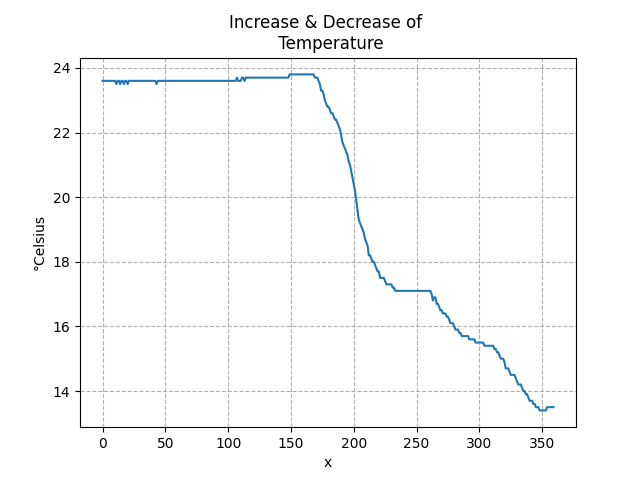
\includegraphics[width=0.49\textwidth]{plot.png}
\caption{Plot des Temperatur Anstiegs und der Abfall}
\label{fig:decrease}
\end{center}
\end{figure}
\begin{figure}[!h]
\begin{center}
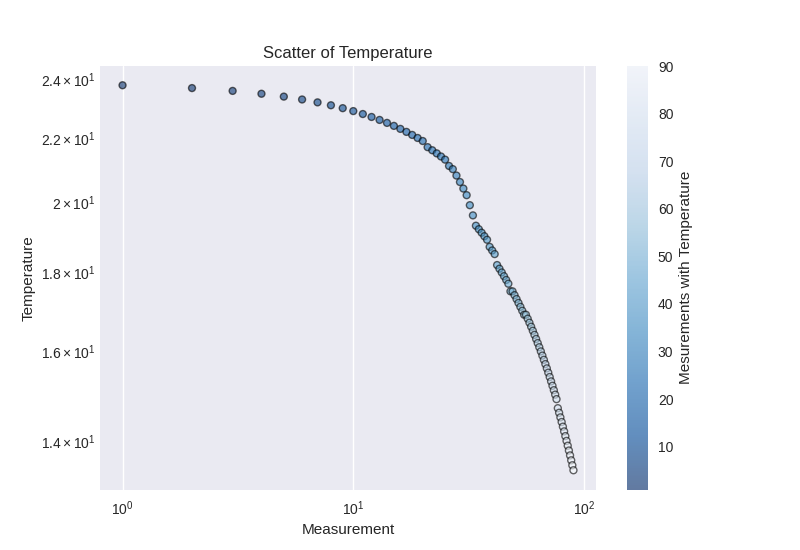
\includegraphics[width=0.53\textwidth]{scatter.png}
\caption{Scatter Plot des Temperatur Abfalls}
\label{fig:scatter}
\end{center}
\end{figure}
\begin{figure}[!h]
\begin{center}
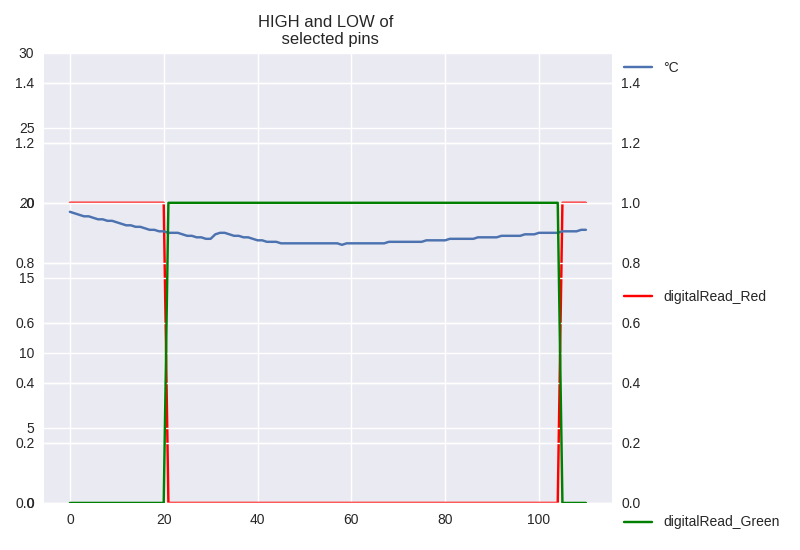
\includegraphics[width=0.53\textwidth]{digitalRead.png}
\caption{HIGH und LOW in einem ersten Test}
\label{fig:highlow}
\end{center}
\end{figure}

\paragraph{Erkenntnisse durch die Daten}
In der Abbildung \ref{fig:decrease} und der Abbildung \ref{fig:scatter} Sieht man wie über eine Gewisse Zeit bei offenen Fenster die Temperatur sinkt. Sommit hatten wir gewissheit, dass der Sensor relativ schnell reagiert und zu gebrauchen ist für das Projekt.
In der Abbildung \ref{fig:highlow} Sieht man zwei Lichter Grüne und Rote, sobald die Temperatur unter 18 $^\circ$C das die Grüne LED auf HIGH war und die Rote LED  auf LOW war, was das Signal ist das die Bedigung für das Einschlafen erreicht ist. Sobald die Temperatur wieder auf 18 $^\circ$C war, nach dem Schliessen des Fensters war die Grüne LED auf LOW und die Rote LED auf HIGH.
Das war die Bestätigung dass das Konzept, welches wir umsetzen wollten aufgehen musste. 
\section{Umsetzung}
\begin{center}
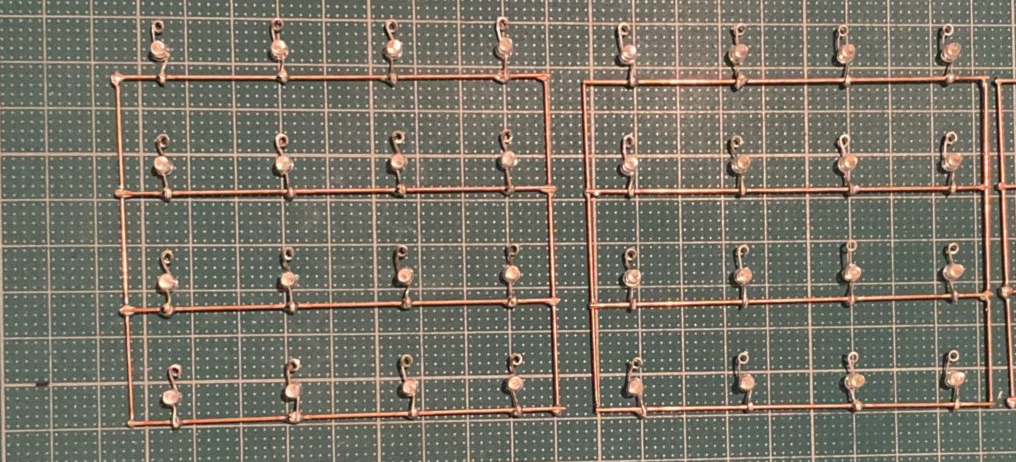
\includegraphics[width=0.53\textwidth]{bilder/layers.jpeg}
\end{center}

\tikzset{darkstyle/.style={circle,draw,fill=gray!40}}
\begin{figure}[hbt!]
\centering
\begin{tikzpicture}
\begin{scope}[every node/.style={circle,thick,draw,fill=gray!40,level distance=200mm,}]
    \node (D48) at (0,0) {D48};
    \node (D46) at (2,0) {D46};
    \node (D44) at (4,0) {D44};
    \node (D42) at (6,0) {D42};
    
    \node (D46) at (2,0) {D46};
    \node (D44) at (4,0) {D44};
    \node (D42) at (6,0) {D42};
    
    \node (D40) at (0,-2) {D40};
    \node (D38) at (2,-2)  {D38};
    \node (D36) at (4,-2) {D36};
    \node (D34) at (6,-2) {D34};
    
    \node (D32) at (0,-4) {D32};
    \node (D30) at (2,-4)  {D30};
    \node (D28) at (4,-4) {D28};
    \node (D26) at (6,-4) {D26};
    
    \node (D24) at (0,-6) {D24};
    \node (D22) at (2,-6)  {D22};
    \node (A5) at (4,-6) {A5};
    \node (A4) at (6,-6) {A4};
    
\end{scope}

\begin{scope}[>={Stealth[black]},
              every node/.style={fill=gray!40,circle,thick},
              every edge/.style={draw=red,very thick}]
     \draw [color=red!100,->,line width=1] (A4) -- (A5);
     \draw [color=red!100,->,line width=1] (A5) -- (D22);
     \draw [color=red!100,->,line width=1] (D22) -- (D24);
     \draw [color=red!100,->,line width=1] (D24) -- (D32);
     \draw [color=red!100,->,line width=1] (D32) -- (D40);
     \draw [color=red!100,->,line width=1] (D40) -- (D48);
     
     \draw [color=red!100,->,line width=1] (D48) -- (D46);
     
     \draw [color=red!100,->,line width=1] (D46) -- (D38);
     \draw [color=red!100,->,line width=1] (D38) -- (D30);
     \draw [color=red!100,->,line width=1] (D30) -- (D22);
     
     \draw [color=red!100,->,line width=1] (D46) -- (D44);
     \draw [color=red!100,<-,line width=1] (D44) -- (D36);
     \draw [color=red!100,<-,line width=1] (D36) -- (D28);
     \draw [color=red!100,<-,line width=1] (D28) -- (A5);
     
     \draw [color=red!100,->,line width=1] (D44) -- (D42);
     \draw [color=red!100,->,line width=1] (D42) -- (D34);
     \draw [color=red!100,->,line width=1] (D34) -- (D26);
     \draw [color=red!100,->,line width=1] (D26) -- (A4);
   
\end{scope}

\end{tikzpicture}
\end{figure}

\section{Resultat}

\section{Evaluation des Resultats}

\section{Gewonnene Erkentnisse}
Dieser Abschnitt besteht nicht nur aus einer Erkenntnis sondern mehreren Erkenntnissen. Deshalb soll in vier Abschnitten folgende Erkentnisse angesprochen werden: 
\begin{enumerate}
\item Die Fähigkeit beziehungsweise die Nützlichkeit unseres Kubus im Alltag,
\item Erkenntnisse über das verwendete Material,
\item Zeitmanagement bis zur Abgabe,
\item Verbesserung in einem nächsten Projekt.
\end{enumerate}

\paragraph{Nützlichkeit im Alltag}
Das unser Kubus im Stande ist auf unterschiedlichliche Temperaturen und eine veränderte Luftfeuchtigkeit zu reagieren ist ausser Frage. Dies wurde in einem Praxistest bei allen drei Gruppenmitgliedern zu Hause getestet. Das bei einer spezifischen Luftfeuchtigkeit \& Temperatur spezifische festgelegte Muster als Feedback angezeigt werden sollen ist vorhanden. \newline \par Ugur hat sich per E-Mail mit, Schlafprofessor Prof. Dr. Björn Rasch in Kontakt gesetzt, um zusätzliche Informationen über die optimale Schlaftemperatur und Luftfeuchtigkeit zu erhalten. Aus einer E-Mail von 03.01.22 wurden drei Punkte deutlich. 
\begin{enumerate}
\item Der Schlaf steht in Korrelation mit der psychologischen Verfassung des Benutzers des Kubus.
\item Die Temperatur für den optimalen Schlaf hängt von dem Microklima unter der Decke ab.
\item Verschiedene Studien kommen zum Schluss, dass 30-50\% oder 30-60\% Luftfeuchtigkeit optimal sind.    
\end{enumerate}
\textbf{Punkt eins} soll keine Stellung genommen werden, da wir über keine fundierte psychologische Ausbildung verfügen, selbst wenn das der Fall wäre, würde dies den Rahmen des Reports sprengen. \\ \textbf{Punkt zwei}, wir sind sicherlich  derselben Meinung, wenn eine Decke zu warm ist, dass der Schlaf dadurch beeinträchtigt wird. Unser Kubus hat aber bei allen drei Mitgliedern dieselbe Erkenntnis hervorgerufen, selbst wenn das Microklima unter der Decke mit der Zeit sich ändert, durch das Lüften in dieser kalten Jahreszeit, das als Konsequenz eine niedrigere Raumtemperatur hervorruft, fällt das Einschlafen mit dem Kubus, bei allen drei Gruppenmitgliedern einfacher. \newline \textbf{Punkt drei}, dass die Luftfeuchtigkeit stimmen muss für den Schlaf/Einschlaf, vorallem in einer kalten Jahreszeit, da kalte Luft relativ trocken ist, kann unser Kubus auch evaluieren. \vspace*{0.2cm}
\par \textbf{Fazit} Die Benutzung des sensor Cubes kann hilfreich sein beim Einschlafen. Allen drei Gruppenmitgliedern hat der sensor Cube aber geholfen. 
 
\paragraph{Das verwendete Material} 
Folgende Komponenten wurden verwendet: 
\begin{enumerate}
\item Kupferdraht
\item Kabel mit einer Litze
\item Arduino UNO 328P $\rightarrow$ Arduino ATMega 2560
\item Lötzinn
\item Flussmittel
\item Schrumpfschlauch
\item Euro-Platine aus Epoxidharz
\item Plexiglas
\item Löt-Station
\item DHT-22
\item LEDs
\item Scharniere
\item Sekundenkleber
\item USB-Stecker - Typ B
\item Multimeter
\item Heissluftföhn
\item Bohrmaschine
\end{enumerate}
In dieser Tabelle sollen nur die Teile aufgelistet werden, welche Probleme bereitet haben. Die Komponenten die nicht in der Tabelle sind, haben \textbf{keine} Probleme verursacht.
\newpage
\begin{table}
    %% \centering % not needed
    \caption{Probleme und Lösungen}
    \rowcolors{1}{}{Gray}
    \begin{tabular}{p{\mylength}|p{\mylength}|p{\mylength}}
        \hline
        \textbf{Komponente} & \textbf{Problem}  &\textbf{Lösung}  \\
        \hline \hline
        Kupferdraht & Der Kupfer draht, welcher bestellt wurde, war beschichtet und ohne das Lötzinn drauf war dieser nicht Leitfähig, die Schicht musste geschmolzen werden oder abgeschliffen werden  & Neuer Kupferdraht wurde erworben\\
        Arduino     & Da wir alle LEDs einzeln ansteuern wollten aber auch den Sensor Verbauen mussten, mussten wir entweder mit i2c arbeiten oder mehr Pins haben& Ugur entschied sich im Sinne der Gruppe auf einen Arduino ATMega 2560 umzustellen        \\
        Lötzinn        & Der Lötzinn, welcher mitgegeben wurde, war relativ alt und ergab beim ersten Löten Zinnkugeln, was optisch nicht ansprechend war & Flussmitttel wurde erworben \\
        Schrumpfschlauch         & Der Schrumpfschlauch der Erworben wurde, passte nicht auf die Verbingdungskabel &  Schrumpfschlauch mit 3mm, welcher auf eine grösse von 1mm schrumpfte wurde Erworben\\
        Euro-Platine aus Epoxidharz   & Bis heute sind wir in der Gruppe nicht einig ob wir die Euro-Platine anders herum hätten verwenden sollen, da der Lötzinn nicht haftete & -      \\
        Plexiglas   & Wir wollten nicht nur ein Platz für unseren Arduino, sondern auch ein Case für den Kubus aus Plexiglas, leider reflektierte das Material die Lichter der LEDs zu stark, somit war nicht erkennbar welche LED rot oder Grün leuchtete. & Verzicht den Kubus in ein Plexiglas gehäuse zu stellen.      \\
        Löt-Station & Die Löt-Spitze, welcher mitgegeben wurde, war oxidiert, somit war es nicht möglich mit dieser Löt-Station zu löten, entweder musste die Lötspitze gereinigt werden oder eine andere Lötstation musste her. & Ugurs Arbeitgeber verlieh eine Professionelle Löt-Station aus.\\
        DHT-22   & Ein Sensor der Mitgelifiert wurde, war defekt. Da wir aber aus Sicherheitsgründen und berichten zwei  bestellt hatten hatten wir ein Backup & Der zusätzliche Sensor wurde verwendet.      \\
        Sekundenkleber & Die Kombination aus Sekundenkleber und Plexiglas verträgt sich nicht gut beim ausprobieren hat Berkan festgestellt das Spuren des Klebers sichtbar werden & Berkan hat trotz der Einschränkung, versucht so sauber wie möglich zu arbeiten\\
        USB-Stecker - Typ B & Der USB-Stecker Typ B war relativ Dick, das wir keine Industrie sind, stehen uns nur bedingte Bohrer zu verfügung, das Loch, welcher für das Kabel gedacht ist, ist ein bisschen Eng. & -  \\
        
        \hline
    \end{tabular}
    \label{table: simulation parameters}
\end{table}

\newpage
\paragraph{Zeitmangement}
Da wir einen Strikten Gant-Chart befolgt haben, wurde alles in der Zeiterledigt, in der denen es zu erreichen war. Wir haben vor dem 1. Januar 2022 genauer am 31.Dezember 2021, ,mit dem sensor Cube fertig. Somit konnten wir viel testen und uns zusätzliche Gedanken machen. Wie zum Beispiel, sollen wir die Luftfeuchtigkeit zusätzlich beachten? Wollen wir ein Case machen? Welche Feedbacks wollen wir? Was ist Sinvoll als Feedback zu nehmen? Wir können behaupten, dass wir die Verwendung des Gant-Charts nochmal in ein selbes Projekt einbinden würden, da dieses den Zeitplan relativ gut eingeteilt hat und immer wieder Überprüfen konnten wo stehen wir.  
\paragraph{Verbesserungswürdig}
Verbesserungswürdig ist in jedem Falle, in einem nächsten Projekt, dass wir durch den Angesprochenen Zeitpuffer, im Paragraph Zeitmangement, vorher definieren würden, ob wir ein Case wollen, welche Materialien verwendet werden sollen. Silvan und Berkan tendieren beide zu Holz, was das Budget erhöhen könnte, aber einfacher wäre das in diesem Projekt einzubinden. Ugur ist der Meinung Plexiglas sieht besser aus, er würde sich einen anderen Klebstoff suchen. Zu dem würden wir uns vorher gedanken machen ob wir genug Pins zur Verfügung stehen, das hat uns zwei Tage gekostet, da die Lieferung bisschen verzögert war. 

\section{Danksagung}
Folgenden Personen/ dem Arbeitgeber soll gedankt werden:
\newline \textbf{Frau Sarah-Lia Andrea Wotke}, sie hat Ugur eine Einführung in das Löten gegeben, er konnte sein Wissen mit Berkan und Silvan teilen. Zu dem hat Sie wichtige Tips gegeben, wir die Kabel isolieren. \newline
\textbf{Herr Prof. Dr. Björn Rasch} an der Universität Fribourg, er hat dem Projekt eine andere Sichtweise gegeben und was beachtet werden sollte.\newline
\textbf{Herr Ilir Ferati} Welcher wichtige Tipps gegeben hat beim Bau des Case und als Ratschlag mitgegeben hat, bitte nächstes Mal Entscheidungen ob ihr ein Case wollt oder nicht früher vor dem Fertigstellen des Kubus fällen.\newline
Als letztes wollen wir uns bei der \textbf{Abteilung Technik des Telebasels} Danken, diese hat uns mit der Zurverfügung Stellung eines Funktionsfähigen Lötkolbens unseren Zeitplan sichergestellt.   

\end{document}
